\documentclass[12pt,a4paper]{article}
\usepackage{geometry,lipsum}
\usepackage{minted}
\usemintedstyle{friendly} % Try 'colorful', 'autumn', or 'tango' for light themes
\usepackage{xcolor}
\definecolor{codebg}{RGB}{245,245,245} % A very light grey background

\setminted{
    bgcolor=codebg,
    fontfamily=tt,
    linenos=true,
    numbersep=5pt,
    frame=lines,
    framesep=2mm,
    breaklines=true,
    fontsize=\small
}
\usepackage{blindtext}
\usepackage[T1]{fontenc}
\usepackage{booktabs}
\usepackage{array}
\usepackage{biblatex}
\usepackage{graphicx}
\renewcommand*{\Rnfont}{\scshape}
\geometry{margin=1.5cm}
\setlength{\parindent}{0.1em}

\begin{document}
\textbf{Data Structures and Algorithms - Bhomik Kinger}
\vspace{\topsep}
\hrule


\section{Arrays}
\subsection{RAM}

Data structure is a way to organize the data in an efficient manner inside the computer component called Random Access Memory (RAM). An array is an ordered collection of contiguous elements, for example [1, 2, 3]. \\
An integer occupies 4 bytes of space in the memory and 1 byte consists of 8 bits. A bit is a smallest unit of measure in computing and can either be represented by 1 or 0. An address and value gets associated upon storing an integer in the RAM. An address is  just a distinct location that each one of the values is stored at.
Each integer occupies 4 bytes of space, so the address are 4 bytes apart. However, a character occupies 1 byte of space in the memory, hence the addresses are 1 byte apart. The size of the data type does not really matter, as long as the address is incremented relative to the size of the data type.

\begin{figure}[h]
    \centering
    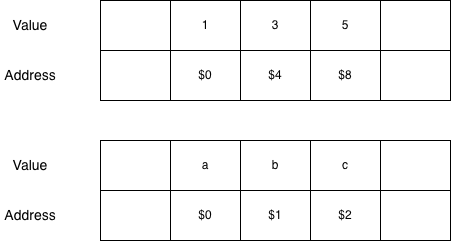
\includegraphics[width=0.5\textwidth]{images/RAM.png}
    \caption{RAM Memory Model}
    \label{fig:RAM Memory Model}
\end{figure}

\subsection{Static Arrays}
In statically typed languages like C++ and Java, arrays have to have an allocated size and type when initialized. These are known as static arrays. \\
Once the array is declared, the size of the array cannot be changed. And once the array is full, it cannot store additional elements. The dynamically typed languages like Python and JavaScript do not have static arrays to begin with.

\subsubsection{Time Complexity}
\begin{table}[h]
\centering
\begin{tabular}{|l|l|l|l|}
\hline
Operation & Big-O Time & Notes \\ \hline
Reading & O(1) & \\ \hline
Insertion & O(n)* & If inserting at the end of the array, O(1) \\ \hline
Deletion & O(n)* & If deleting at the end of the array, O(1) \\ \hline

\end{tabular}
\end{table}

\subsubsection{Code}
\begin{minted}{python}
# Length is the number of elements in the array
# Capacity is the memory allocated for the fixed size array
# O(1) time
def insertEnd(arr, n, length, capacity):
    if length < capacity:
        arr[length] = n

# Soft delete - overwriting the last element to 0
# [1, 3, 4, 5]
# [1, 3, 4, 0]
# O(1) time
def removeEnd(arr, length):
    # check if array is not empty
    if length >= 1:
        arr[length - 1] = 0

# [1, 3, 5] (insert 4 at idx 1) -> [1, 4, 3, 5] (shift the elemnts by 1 pos to the right)
# O(n) time
def insertMiddle(arr, i, n, length):
    # shift the elements by 1 pos to the right (length - 1, i)
    for idx in range(length, i, -1):
        arr[idx] = arr[idx - 1]
    # insert the element at ith index
    arr[i] = n

# [1, 3, 5, 6] (remove the element at 2nd pos) -> [1, 3, 6, ?] (shift the elements to the left)
# O(n) time
def removeMiddle(arr, i, length):
    # shift the elements to the left by 1 pos
    for idx in range(i, length - 1):
        arr[idx] = arr[idx + 1]

# O(n) time
def printArr(arr, capacity):
    for i in range(capacity):
        print(arr[i])
\end{minted}


\subsection{Dynamic Arrays}
Dynamic Arrays (aka resizable arrays) can change their size during the runtime of the program. The size of the dynamic array can be increased as we add more elements into it. Programming languages like JavaScript and Python only have dynamic arrays.

\begin{minted}{python}
class DynamicArray:
    
    def __init__(self, capacity: int):
        self.capacity = capacity
        self.arr = [0] * capacity
        self.size = 0

    # O(1) time
    def get(self, i: int) -> int:
        # assuming i index is valid
        return self.arr[i]

    # O(1) time
    def set(self, i: int, n: int) -> None:
        # assuming i index is valid
        self.arr[i] = n

    # O(1) time (Amortized)
    def pushback(self, n: int) -> None:
        if self.size == self.capacity:
            self.resize()

        self.arr[self.size] = n
        self.size += 1

    # O(1) time
    def popback(self) -> int:
        self.size -= 1
        return self.arr[self.size]

    # O(n) time
    def resize(self) -> None:
        self.capacity = 2 * self.capacity
        self.newArr = [0] * self.capacity
        for i in range(self.size):
            self.newArr[i] = self.arr[i]
        self.arr = self.newArr

    # O(1) time
    def getSize(self) -> int:
        return self.size
    
    # O(1) time
    def getCapacity(self) -> int:
        return self.capacity
\end{minted}
\subsubsection{Time Complexity}
\begin{table}[h]
\centering
\begin{tabular}{|l|l|l|l|}
\hline
Operation & Big-O Time & Notes \\ \hline
Access & O(1) & \\ \hline
Insertion & O(1)* & O(n) if inserting in the middle of array \\ \hline
Deletion & O(1)* & O(n) if deleting an element in the middle of array \\ \hline

\end{tabular}
\end{table}




\subsection{Singly Linked List}
????

\begin{minted}{python}
???
\end{minted}
\subsubsection{Time Complexity}
\begin{table}[h]
\centering
\begin{tabular}{|l|l|l|l|}
\hline
Operation & Big-O Time & Notes \\ \hline
?? & O(?) & \\ \hline
?? & O(?) &  \\ \hline
?? & O(?) & \\ \hline

\end{tabular}
\end{table}
\end{document}


